\documentclass[10pt,a4wide]{article}
\usepackage[english]{babel}
\usepackage{a4wide}
\usepackage{graphicx}
\usepackage{graphics}
\usepackage{fancyheadings}
\pagestyle{fancy}

\bibliographystyle{plain}

\lhead{{\scriptsize kaneton project}}
\rhead{k2 subject}
\rfoot{\scriptsize EPITA System Lab}

\title{kaneton2}

\author{Julien Quintard - \small{quinta\_j@epita.fr} \\
        Jean-Pascal Billaud - \small{billau\_j@epita.fr} \\ \\
	\small{last updated by} \\
	Julien Quintard - \small{quinta\_j@epita.fr}}

\date{\today}

\begin{document}
\maketitle

\section{Informations}

\begin{tabular}{p{7cm}l}

Date de rendu: & Lundi 14 Mars 2005 \`a 23h42 \\
Dur\'ee du projet: & 2 semaines \\
Nom du fichier de rendu: & k2.tar.gz \\
Responsable du projet: & Julien Quintard - \small{quinta\_j@epita.fr} \\
                       & Jean-Pascal Billaud - \small{billau\_j@epita.fr} \\
Newsgroups d\'edi\'es: & epita.kaneton, epita.adm.sr \\
Langages: & asm, C \\
Architectures: & Intel 32-bit \\
Nombre de personnes par groupes: & 3 \`a 5

\end{tabular}

\section{Introduction}

\paragraph{}

Le but de ce projet est de mettre en place un certain nombre de gestionnaires.

\paragraph{}

Le but du projet pr\'ec\'edent \'etait de mettre en place un environnement
propice \`a l'ex\'ecution du kernel. Au lancement du kernel, celui-ci
sait qu'il est mapp\'e en m\'emoire haute, qu'il dispose de la segmentation
et de la pagination et qu'il peut acc\'eder aux structures de donn\'ees.

\paragraph{}

A pr\'esent le kernel doit \^etre capable de traiter les interruptions
mat\'erielles, les exceptions et les interruptions logicielles. Ainsi,
vous devrez d\'evelopper une API permettant d'int\'eragir avec les
p\'eriph\'eriques.

\paragraph{}

De plus, un gestionnaire de m\'emoire physique sera indispensable pour allouer
et lib\'erer de la m\'emoire physique.

\section{Travail Demand\'e}

\paragraph{}

Le projet consiste en la mise en place de plusieurs gestionnaires. Pour chacun
d'entre eux nous vous demandons de pr\'evoir une partie ind\'ependante du
processeur ainsi qu'une partie d\'ependante mais cela sera expliqu\'e
dans la section Portabilit\'e.

\paragraph{}

Voici les \'etapes \`a respecter:

\begin{enumerate}
\item gestionnaire d'espaces d'adressage.
\item gestionnaire de segmentation.
\item gestionnaire de m\'emoire physique.
\item gestionnaire de traps.
\item gestionnaire d'interruptions et d'exceptions.
\item gestion du PIC.
\item d\'eveloppement d'un driver clavier.
\item d\'eveloppement d'un driver timer.
\item D\'eveloppement d'un interpr\'eteur de d\'emonstration qui lit
      une commande au clavier et effectue une op\'eration.
\end{enumerate}

\paragraph{}

Une fois ces op\'erations effectu\'ees vous pourriez d\'ej\`a consid\'erer
avoir un kernel presque complet. Nous pourrions dans tous les cas dire
que le plus d\^ur est fait.

\section{Interfaces}

\paragraph{}

Nous vous rappellons que vous \^etes libres d'utiliser une autre
interface. Dans ce cas il vous sera demander une documentation expliquant
vos choix tr\`es pr\'ecis\'ement. Sans celle-ci votre travail serait
consid\'er\'e comme inachev\'e et non concordant avec le sujet.

\paragraph{}

Les fonctions des interfaces retournent \textbf{0} si tout c'est
pass\'e correctement ou \textbf{-1} s'il s'est produit une erreur.
Il vous est autoris\'e d'\'etendre la gestion des erreurs en
renvoyant une valeur n\'egative s'il s'est produit une erreur,
cette valeur correspondant \`a un type d'erreur pr\'ecis. Cette norme
sera suivie pour tous les projets, de k0 \`a kn.

\subsection{Console}

Nous vous laissons le choix de l'interface de la gestion de la console.

\paragraph{}

Toutefois la console devra permettre:

\begin{itemize}
\item l'affichage d'un caract\`ere: \textbf{cons\_print\_char}().
\item l'affichage d'une chaine de caract\`eres: \textbf{cons\_print\_string}().
\item l'affichage d'un nombre avec une base donn\'ee:
      \textbf{cons\_print\_num}().
\item l'affichage d'une chaine de format via la fonction \textbf{printf}() qui
      devra se trouver bien entendu dans la libc.
\item le scrolling.
\item l'affichage du backspace, en d'autres termes l'effacement
      d'un caract\`ere.
\item l'effacement complet de la console.
\item la red\'efinition des attributs de la console \`a n'importe quel moment.
\item la gestion du curseur, celui-ci \'etant controll\'e via I/O ports.
\end{itemize}

\subsection{Espace d'adressage}

\paragraph{}

Vous devez fournir une interface destin\'ee \`a la gestion des
espaces d'adressage.

\paragraph{}

Cette partie du syst\`eme sera compl\'et\'ee dans les projets suivants,
principalement dans k3, qui se chargera de toute la partie virtuelle.

\paragraph{}

Un espace d'adressage est compos\'e d'une structure de donn\'ees destin\'ee
\`a contenir suffisamment d'informations pour d\'ecrire la m\'emoire
utilis\'ee par un processus, que cette m\'emoire soit physique, virtuelle,
mapp\'ee, non mapp\'ee etc..

\paragraph{}

\hspace{1.5cm}int \textbf{as\_init}(void);

\paragraph{}

Cette fonction initialise la gestion des espaces adressage.

\paragraph{}

\hspace{1.5cm}int \textbf{as\_rsv}(t\_asid \textbf{*asid});

\paragraph{}

Cette fonction r\'eserve un espace d'adressage, c'est-\`a-dire une structure
de donn\'ees d\'ecrivant un espace d'adressage. La fonction se contente
de r\'eserver et d'initialiser la structure de donn\'ees puis de retourner
son identifiant.

\paragraph{}

\hspace{1.5cm}int \textbf{as\_get}(t\_asid \textbf{asid},
                                   t\_as \textbf{*as});

\paragraph{}

Cette fonction retourne l'adresse de la structure d\'ecrivant l'espace
d'adressage \`a partir de son identifiant. Cette fonction peut \^etre
consid\'er\'ee comme priv\'ee dans le sens o\`u seules les fonctions
influant sur les espaces d'adressage devraient y faire appel:
\textbf{pm\_rsv}(), \textbf{vm\_rel} etc..

\paragraph{}

Pour rappel, les gestionnaires d'espace d'adressage, de m\'emoire physique
et de m\'emoire virtuelle fonctionnent ensemble pour garder traces des
allocations de m\'emoire. Tout cela se caract\'erisant par une manipulation
de deux types de structure: \textbf{t\_pm} qui repr\'esente l'\'etat g\'eneral
de la m\'emoire physique du syst\`eme et \textbf{t\_as} qui d\'ecrit
un espace d'adressage; chaque t\^ache ayant th\'eoriquement un espace
d'adressage.

\paragraph{}

\hspace{1.5cm}int \textbf{as\_rel}(t\_asid \textbf{asid});

\paragraph{}

Cette fonction lib\`ere l'espace d'adressage sp\'ecifi\'e.

\paragraph{}

\hspace{1.5cm}int \textbf{as\_clear}(void);

\paragraph{}

Cette fonction d\'etruit tous les espaces d'adressage.

\subsection{Segments}

\paragraph{}

Nous vous demandons de d\'evelopper une interface pour la gestion des
segments. Comme nous l'avons vu en cours, le gestionnaire
de segmentation sur processeur IA-32 inclue la gestion des segments
m\'emoire ainsi que la gestion des contextes processeur TSS.

\paragraph{}

Cette partie sera consid\'er\'ee comme \'etant la partie ``machine
dependent'' de la gestion de la m\'emoire physique. De ce fait votre
gestionnaire de segments pourra tout \`a fait coller au processeur
Intel, et c'est d'ailleurs ce que nous allons tenter de faire.
De plus un syst\`eme ne disposant pas de notion de segments ne souffrira
pas de cette impl\'ementation puisqu'il lui suffira de faire comme bon
lui semble.

\paragraph{}

Le but ici est de proposer une interface pour pouvoir manipuler principalement
les segments m\'emoire car les contextes processeurs TSS ne seront pas
utilis\'es dans kaneton.

\paragraph{}

Voici donc l'interface que nous vous proposons concernant la
gestion des segments.

\paragraph{}

Notez bien que chaque op\'eration sur les segments doit \^etre
visible imm\'ediatement une fois l'op\'eration termin\'ee.

\paragraph{}

\hspace{1.5cm}int \textbf{seg\_init}(void);

\paragraph{}

Cette fonction initialise la gestion des segments.

\paragraph{}

\hspace{1.5cm}int \textbf{seg\_add}(t\_paddr \textbf{start},
                                    t\_paddr \textbf{size},
                                    t\_pl \textbf{pl},
                                    t\_segtype \textbf{type},
                                    t\_segid \textbf{*segid});

\paragraph{}

Cette fonction se contente d'ajouter un segment et de le mettre en
place en l'indiquant au processeur.

\paragraph{}

L'argument \textbf{pl} repr\'esente le ``Privilege Level'': PL\_KERNEL,
PL\_SERVICE, PL\_USER mais \'egalement PL\_EXEC, PL\_READ, PL\_WRITE
alors que \textbf{type} repr\'esente le type du segment: SEG\_MEM, SEG\_TSS.

\paragraph{}

La fonction devra remplir le param\`etre \textbf{segid} avec l'identifiant
du segment.

\paragraph{}

\hspace{1.5cm}int \textbf{seg\_modify}(t\_segid \textbf{segid},
                                       t\_paddr \textbf{start},
                                       t\_paddr \textbf{size},
                                       t\_pl \textbf{pl},
                                       t\_segtype \textbf{type});

\paragraph{}

Cette fonction modifie le segment identifi\'e via le param\`etre
\textbf{segid}.

\paragraph{}

\hspace{1.5cm}int \textbf{seg\_remove}(t\_segid \textbf{segid});

\paragraph{}

Cette fonction efface un segment en le retirant de la liste des segments
utilis\'es.

\paragraph{}

\hspace{1.5cm}int \textbf{seg\_clear}(void);

\paragraph{}

Cette fonction d\'etruit tous les segments pr\'esents.

\paragraph{}

Il est \`a noter qu'\'etant donn\'e que le gestionnaire de segments
renvoie des identifiants, cela implique que ce gestionnaire est capable
de retrouver la structure de donn\'ees \`a partir de l'identifiant. Cet aspect
se retrouvera dans chaque gestionnaire utilisant des identifiants. \`A vous
donc de mettre en place un m\'ecanisme pour retrouver un objet \`a partir
de son identifiant.

\paragraph{}

Il est important de bien comprendre que l'utilisant d'identifiants pour cette
partie est absolument inutile puisque faisant partie de la partie ``machine
dependent''. N\'eanmoins celle-ci est pr\'esente pour que vous vous
familiarisiez avec ce type de gestionnaires.

\subsection{M\'emoire physique}

\paragraph{}

Il vous est \'egalement demand\'e de fournir une interface pour
l'utilisation de la m\'emoire physique. Comme nous venons de le voir,
la partie ``machine dependent'' du gestionnaire de m\'emoire physique
sera g\'er\'ee par le gestionnaire de segments. Voyons d\'esormais
l'interface de la partie ``machine independent''.

\paragraph{}

Libre \`a vous d'utiliser l'algorithme que vous estimez le plus performant,
propre, facile \`a impl\'ementer: bitmap, bitmap \'evolu\'e, zones etc.. via
la structure de donn\'ees appropri\'ee: tableau, liste chain\'ee, arbre etc..

\paragraph{}

\hspace{1.5cm}int \textbf{pm\_init}(t\_paddr \textbf{start},
                                    t\_paddr \textbf{size});

\paragraph{}

Cette fonction se charge d'initialiser le gestionnaire de m\'emoire physique.

\paragraph{}

\hspace{1.5cm}int \textbf{pm\_rsv}(t\_asid \textbf{asid},
                                   t\_paddr \textbf{*addr},
                                   t\_paddr \textbf{npages},
                                   t\_pmflags \textbf{flags});

\paragraph{}

Cette fonction a pour but d'allouer un nombre donn\'e de pages contig\"ues
de m\'emoire physique.

\paragraph{}

L'argument \textbf{*addr} doit \^etre rempli par la fonction, indiquant
l'adresse de la zone allou\'ee. L'argument \textbf{flags} indique les options
d'allocation: PM\_FLAG\_ANY, PM\_FLAG\_DMA etc..

\paragraph{}

L'allocateur de m\'emoire physique peut utiliser l'asid et les
propri\'et\'es sur les zones pour fusionner celles-ci, all\'egeant
la structure de donn\'ees utilis\'ee pour la gestion de la m\'emoire.

\paragraph{}

Cette op\'eration devra \'egalement modifier la structure de donn\'ees
d\'ecrivant l'espace physique dans l'\textbf{as} sp\'ecifi\'e, cela
dans l'unique but de garder les structures coh\'erentes.

\paragraph{}

\hspace{1.5cm}int \textbf{pm\_rel}(t\_asid \textbf{asid},
                                   t\_paddr \textbf{addr},
                                   t\_paddr \textbf{npages});

\paragraph{}

Cette fonction se contente de lib\'erer un certain nombre
de pages de m\'emoire physique.

\paragraph{}

M\^eme chose pour cette fonction, il faudra \'egalement intervenir sur
l'\textbf{as} sp\'ecifi\'e.

\paragraph{}

\hspace{1.5cm}int \textbf{pm\_flush}(t\_asid \textbf{asid});

\paragraph{}

Cette fonction lib\`ere toute la m\'emoire physique que l'espace d'adressage
\textbf{asid} utilise.

\paragraph{}

\hspace{1.5cm}int \textbf{pm\_clear}(void);

\paragraph{}

Cette fonction r\'einitialise la gestion de la m\'emoire physique en lib\'erant
les pages utilis\'ees.

\subsection{Interruptions/Exceptions}

\paragraph{}

La gestion des interruptions et des exceptions sur processeur Intel se fait
gr\^ace \`a une table nomm\'ee IDT.

\paragraph{}

Voici l'interface a utiliser pour la gestion des interruptions et exceptions
Intel.

\paragraph{}

Cette partie repr\'esente la partie totalement ``machine dependent'' de la
gestion des traps mais fera \'egalement partie de la partie
``machine dependent'' des messages. Pensez \`a organiser le code convenablement
pour \'eviter la duplication de code inutilement.

\paragraph{}

\hspace{1.5cm}int \textbf{int\_init}(void);

\paragraph{}

Cette fonction initialise la gestion des interruptions.

\paragraph{}

\hspace{1.5cm}int \textbf{int\_add}(u\_int8\_t \textbf{entry},
                                    t\_inttype \textbf{type},
                                    t\_segid \textbf{segid},
                                    t\_pl \textbf{pl},
                                    t\_vaddr \textbf{handler});

\paragraph{}

Cette fonction ajoute un handler sur le vecteur d'interruption \textbf{entry}.
Le param\`etre \textbf{type} repr\'esente le type de handler \`a g\'erer:
INT\_INTGATE, INT\_TRAPGATE, INT\_TASKGATE ou INT\_CALLGATE. L'argument
\textbf{segid} repr\'esente le segment contenant le handler et \textbf{pl}
repr\'esente les privil\`eges de l'interruption.

\paragraph{}

\`A savoir que nous utiliserons seulement le type INT\_INTGATE, mais
ce point tr\`es pr\'ecis sera explicit\'e ult\'erieurement.

\paragraph{}

\hspace{1.5cm}int \textbf{int\_modify}(u\_int8\_t \textbf{entry},
                                       t\_inttype \textbf{type},
                                       t\_segid \textbf{segid},
                                       t\_pl \textbf{pl},
                                       t\_vaddr \textbf{handler});

\paragraph{}

Cette fonction modifie une interruption d\'ej\`a enregistr\'ee.

\paragraph{}

\hspace{1.5cm}int \textbf{int\_remove}(u\_int8\_t \textbf{entry});

\paragraph{}

Cette fonction efface une entr\'ee de la table d'interruptions.

\paragraph{}

\hspace{1.5cm}int \textbf{int\_clear}(void);

\paragraph{}

Cette fonction r\'einitialise la gestion des interruptions.

\subsection{Traps}

\paragraph{}

La gestion des interruptions est tr\`es importante car elle va permettre
\`a votre kernel de recevoir des messages provenant des p\'eriph\'eriques.

\paragraph{}

Le concept d'interruption et d'exception est encore une fois trop
sp\'ecifique \`a Intel. Il pourrait exister des architectures sur
lesquelles ces concepts sont confondus. Pour cette raison les exceptions
comme les interruptions seront consid\'er\'ees en tant que \textbf{trap}.

\paragraph{}

Une \textbf{trap} repr\'esentant une porte d'entr\'ee vers une t\^ache pour
les \'ev\`enements mat\'eriels, que ce soit un \'ev\`enement provenant
d'un p\'eriph\'erique comme du processeur.

XXX trap sont aussi des portes pour les messages ... enfin il faut trouver
    comment faire pour envoyer un message vers un identifiant alors que tu
    veux certainement l envoyer a une personne. en realite il faut mettre
    en valeur des cas concrets. style hop communication entre deux process
    pour faire tel trucs. de meme genre un truc qui veut des stats sur le
    reseau, il devra y avoir un process qui se registera sur la meme trap
    que celle du driver reseau pour recevoir les stats. les questions sont
    comment retrouver les traps, donc comment retrouver les task etc..

\paragraph{}

La gestion de message ne se base pas sur les traps mais utilise un autre
m\'ecanisme. Les traps sont exclusivement r\'es\`erv\'ees \`a l'acheminement
d'\`ev\`enement que nous nommeront ``mat\'eriels''.

\paragraph{}

Il faut tout de m\^eme savoir que chaque \'ev\`enement mat\'eriel sera
transmis au handler sous forme de message. Lorsque vous ajouterez donc une
trap sur tel \'ev\`enement, pensez que la thread qui sera r\'eveill\'ee
devra \^etre capable de traiter un message en entr\'ee.

\paragraph{}

\hspace{1.5cm}int \textbf{trap\_init}(void);

\paragraph{}

Cette fonction initialise la gestion des traps.

\paragraph{}

\hspace{1.5cm}int \textbf{trap\_add}(t\_hwid \textbf{hwid},
                                     t\_thrid \textbf{thrid},
                                     t\_trapid \textbf{*trapid});

\paragraph{}

Cette fonction ajoute une trap qui d\'eclenchera l'ex\'ecution de la thread
\textbf{thrid} lorsque l'\'ev\`ement \textbf{hwid} se manifestera.

\paragraph{}

Nous vous conseillons de faire en sorte qu'une fois la trap trait\'ee il
soit possible d'en recevoir une nouvelle. Ceci n'est qu'un conseil qu'il
faudra prendre en compte lors de l'\'elaboration du code de vos handlers
de messages.

\paragraph{}

Le param\`etre \textbf{hwid} peut sembler flou. En effet cet argument
repr\'esente un identifiant de ressource. Dans le cas d'Intel nous pouvons
imaginer que vos drivers vont interroger le controlleur PCI pour obtenir
l'IRQ correspondant \`a ce p\'eriph\'erique. Cet IRQ sera donc
transmis en tant que \textbf{hwid}.

\paragraph{}

Le fait est que peu importe ce que repr\'esente \textbf{hwid}. Le plus
important \'etant qu'une norme soit d\'efinie. Dans tous les cas nous pouvons
dire que l'argument \textbf{hwid} repr\'esente un identifiant de ressource
et que cet identifiant est assign\'e par le mat\'eriel. Le tout \'etant
que la partie ``machine dependent'' de votre kernel soit capable de mettre
en place des traps \`a partir de cet identifiant de ressource.

\paragraph{}

\hspace{1.5cm}int \textbf{trap\_modify}(t\_trapid \textbf{trapid},
                               	        t\_thrid \textbf{thrid});

\paragraph{}

Cette fonction permet de modifier une trap d\'ej\`a enregistr\'ee.

\paragraph{}

\hspace{1.5cm}int \textbf{trap\_remove}(t\_trapid \textbf{trapid});

\paragraph{}

Permet d'effacer la trap du gestionnaire de traps.

\paragraph{}

\hspace{1.5cm}int \textbf{trap\_enable}(t\_trapid \textbf{trapid});

\paragraph{}

Permet d'activer la gestion de cette trap. \`A vous de d\'ecider si jamais
l'installation d'une trap l'active par d\'efaut.

\paragraph{}

\hspace{1.5cm}int \textbf{trap\_disable}(t\_trapid \textbf{trapid});

\paragraph{}

Permet de d\'esactiver la gestion de cette trap.

\subsection{Clavier}

\paragraph{}

L'interface du driver clavier est laiss\'ee au choix du groupe pour certaines
raisons, la premi\`ere \'etant le fait que cette interface devra \'evoluer
avec le temps.

\paragraph{}

Inutile donc de s'acharner sur la mod\'elisation. N\'eanmoins nous vous
conseillons de faire un driver complet pour ne pas avoir de probl\`emes
plus tard.

\subsection{PIC}

\paragraph{}

Le PIC est encore une fois un \'el\'ement trop sp\'ecifique. Pour cette
raison la gestion du PIC sera incluse dans la partie ``machine dependent''.

\paragraph{}

Tous les appels \`a l'interface PIC seront faits \`a partir du gestionnaire
de traps.

\paragraph{}

\hspace{1.5cm}int \textbf{pic\_init}(void);

\paragraph{}

Cette fonction initialise la gestion du PIC.

\paragraph{}

\hspace{1.5cm}int \textbf{pic\_enable}(t\_hwid \textbf{hwid});

\paragraph{}

Cette fonction active l'interruption \textbf{hwid}.

\paragraph{}

\hspace{1.5cm}int \textbf{pic\_disable}(t\_hwid \textbf{hwid});

\paragraph{}

Cette fonction d\'esactive l'interruption \textbf{hwid}.

\paragraph{}

\hspace{1.5cm}int \textbf{pic\_clear}(void);

\paragraph{}

Cette fonction r\'einitialise la gestion du PIC.

\subsection{Timer}

L'interface du timer est laiss\'ee au choix du groupe.

\paragraph{}

Le but \'etant de g\'erer les interruptions timer et de retenir le nombre
de \textbf{ticks} \'ecoul\'es.

\newpage

\section{Visualisation}

\paragraph{}

Voici une visualisation de l'interaction entre la partie
``machine independent'' et la partie ``machine dependent''

\begin{figure}[h]
\centerline{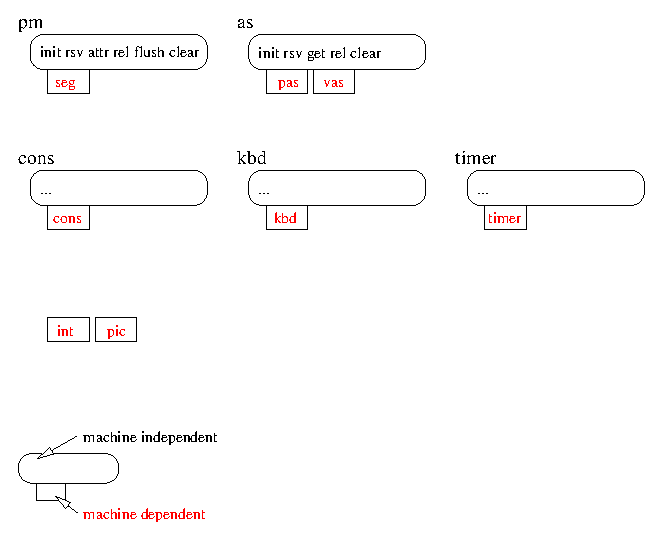
\includegraphics{figures/visualisation.eps}}
\end{figure}

Nous pouvons distinguer trois sections:

\subsection{``Machine independent''}

\paragraph{}

La premi\`ere section est enti\`erement ind\'ependante de l'architecture et
est compos\'ee du gestionnaire de m\'emoire physique et du gestionnaire
d'espace d'adressage.

\paragraph{}

En effet le gestionnaire de m\'emoire physique se contente de g\'erer
une zone de m\'emoire avec des propri\'et\'es sur certaines zones: utilis\'ee,
inutilis\'ee, partag\'ee etc..

\subsection{Interfaces}

\paragraph{}

La seconde section de la figure est compos\'ee des interfaces de communication
entre la partie d\'ependante de l'architecture et la partie ind\'ependante.

\paragraph{}

Ainsi une partie du gestionnaire de traps sera contenue dans la partie
``machine independent'' car celui-ci n'a pas besoin de connaitre le
fonctionnement des traps au niveau hardware. En revanche une partie
du gestionnaire de traps sera contenue dans la partie ``machine dependent''
car celle-ci aura comme but de mettre en place une trap au niveau hardware.

\paragraph{}

Ces interfaces seront toujours compos\'ees de deux parties bien distinctes:
une partie destin\'ee \`a la mise en place hardware du concept en
question et une partie plus haut niveau destin\'ee \`a la gestion du concept
sans se pr\'eoccuper de l'impl\'ementation.

\subsection{``Machine dependent''}

\paragraph{}

La troisi\`eme section est enti\`erement compos\'ee de code li\'e \`a
l'architecture, dans notre cas IA-32.

\paragraph{}

En effet le concept d'interruption n'est pas connu de la partie
``machine independent'', seulement de la partie ``machine dependent'' des
traps. M\^eme chose pour le PIC qui pourrait ne pas exister sur
certaines architectures.

\subsection{Hi\'erarchie}

\paragraph{}

Comme vous pouvez le constater, il existe une hi\'erarchie.

\paragraph{}

La couche ``machine independent'' d\'el\`egue du travail via les interfaces
aux couches ``machine dependent''.

\paragraph{}

Cette hi\'erarchie ne doit jamais \^etre bris\'ee sans quoi le mod\`ele
deviendra incoh\'erent.

\section{Types}

XXX expliquer les types, sturctures etc.. genre ceux dependent ..

\section{Bonus}

\paragraph{}

Voici les bonus de ce projet.

\subsection{Sharing}

Un ajout int\'eressant dans la gestion de la m\'emoire physique sera
de permettre le partage de pages physiques.

\paragraph{}

Votre gestionnaire de m\'emoire physique devra donc garder une trace sur
le nombre de personnes utilisant une page ou une zone de pages physiques.

\paragraph{}

Lorsqu'une page partag\'ee par plusieurs espaces d'adressage est lib\'er\'ee
il faut d\'ecr\'ementer le nombre d'espaces d'adressage l'utilisant. Si ce
compteur tombe \`a zero alors la page peut \^etre lib\'er\'ee.

\paragraph{}

Une optimisation sera d'introduire un syst\`eme de protection pour que
seuls les espaces d'adressage autoris\'es puissent mapper cette page
partag\'ee.

\subsection{Tty}

Il pourrait \^etre int\'eressant de disposer de diff\'erents tty, c'est \`a
dire des couples console - clavier diff\'erent.

\paragraph{}

Il vous sera donc demander de fournir un interface compl\`ete pour la
manipulation des tty.

\end{document}
